\documentclass[../main.tex]{subfiles}

\begin{document}

\section{Exercise 2.1}

Code:

\begin{lstlisting}
(define (gcd a b)
  (define (gcd-non-negative a b)
    (if (= b 0)
        a
        (gcd-non-negative b (remainder a b))))
  (cond ((< b 0) (gcd a (- 0 b)))
        ((< a 0) (gcd (- 0 a) b))
        (else (gcd-non-negative a b))))

(define (make-rat n d)
  (if (< d 0)
      (make-rat (- 0 n) (- 0 d))
      (let ((g (gcd n d)))
        (cons (/ n g) (/ d g)))))
\end{lstlisting}

Tests:

\begin{lstlisting}
(make-rat 9 6)   ; (3 . 2) expected
(make-rat 9 -6)  ; (-3 . 2) expected
(make-rat -9 6)  ; (-3 . 2) expected
(make-rat -9 -6) ; (3 . 2) expected
\end{lstlisting}

\section{Exercise 2.2}

Code:

\begin{lstlisting}
;; point definition
(define (make-point x y)
  (cons x y))
(define (x-point point)
  (car point))
(define (y-point point)
  (cdr point))

;; segment definition
(define (make-segment start end)
  (cons start end))
(define (start-segment segment)
  (car segment))
(define (end-segment segment)
  (cdr segment))
(define (midpoint-segment segment)
  (define (average x y)
    (/ (+ x y) 2.0))
  (let ((start (start-segment segment))
        (end (end-segment segment)))
    (make-point (average (x-point start)
                         (x-point end))
                (average (y-point start)
                         (y-point end)))))
\end{lstlisting}

Tests:

\begin{lstlisting}
(midpoint-segment (make-segment (make-point 1.0 2.0)
                                (make-point 4.0 3.0))) ; (2.5 . 2.5) expected
(midpoint-segment (make-segment (make-point 1.0 2.0)
                                (make-point 3.0 4.0))) ; (2.0 . 3.0) expected
\end{lstlisting}

\section{Exercise 2.3}

Code:

\begin{lstlisting}
;; one version of rectangle
(define (make-rect top-left bottom-right)
  (cons top-left bottom-right))
(define (top-left rect)
  (car rect))
(define (bottom-right rect)
  (cdr rect))
(define (width rect)
  (- (x-point (bottom-right rect))
     (x-point (top-left rect))))
(define (height rect)
  (- (y-point (bottom-right rect))
     (y-point (top-left rect))))

;; another version of rectangle
(define (make-rect top-left width height)
  (cons top-left (cons width height)))
(define (top-left rect)
  (car rect))
(define (width rect)
  (car (cdr rect)))
(define (height rect)
  (cdr (cdr rect)))

;; rect procedures
(define (perimeter rect)
  (* 2 (+ (width rect) (height rect))))
(define (area rect)
  (* (width rect) (height rect)))
\end{lstlisting}

\section{Exercise 2.4}

By evaluating \lstinline{(car (cons x y))} using
 applicative-order strategy, it can be verified
 that \lstinline{(car (cons x y))} yields
 \lstinline{x} for any object \lstinline{x} and
 \lstinline{y}:

\begin{lstlisting}
(car (cons x y)) ->
(car (lambda (m) (m x y))) ->
((lambda (m) (m x y)) (lambda (p q) p)) ->
((lambda (p q) p) x y) ->
x
\end{lstlisting}

The same result can also be obtained using
 normal-order strategy:

\begin{lstlisting}
(car (cons x y)) ->
((cons x y) (lambda (p q) p)) ->
((lambda (m) (m x y)) (lambda (p q) p)) ->
((lambda (p q) p) x y) ->
x
\end{lstlisting}

The corresponding definition of \lstinline{cdr}:

\begin{lstlisting}
(define (cdr z)
  (z (lambda (p q) q)))
\end{lstlisting}

\section{Exercise 2.5}

Code:

\begin{lstlisting}
(define (cons x y)
  (* (expt 2 x) (expt 3 y)))
(define (car z)
  (define (car-iter z sum)
    (if (= (remainder z 2) 0)
        (car-iter (/ z 2) (+ 1 sum))
        sum))
  (car-iter z 0))
(define (cdr z)
  (define (cdr-iter z sum)
    (if (= (remainder z 3) 0)
        (cdr-iter (/ z 3) (+ 1 sum))
        sum))
  (cdr-iter z 0))
\end{lstlisting}

\section{Exercise 2.6}

Code:

\begin{lstlisting}
(define one (lambda (f) (lambda (x) (f x))))
(define two (lambda (f) (lambda (x) (f (f x)))))
(define (add a b)
  (lambda (f) (lambda (x) ((a f) ((b f) x)))))
\end{lstlisting}

Tests:

\begin{lstlisting}
(define (incre x) (+ x 1))
((one incre) 0)            ; 1 expected
((two incre) 0)            ; 2 expected
(define four (add two two))
((four incre) 0)           ; 4 expected
(((add four two) incre) 0) ; 6 expected
\end{lstlisting}

\section{Exercise 2.7}

Code:

\begin{lstlisting}
(define (upper-bound interval)
  (car interval))
(define (lower-bound interval)
  (cdr interval))
\end{lstlisting}

\section{Exercise 2.8}

The difference of two intervals is the
 sum of the first interval and the opposite
 of the second interval.

Code:

\begin{lstlisting}
(define (sub-interval x y)
  (define (neg-interval x)
    (make-interval (- 0 (upper-bound x)) (- 0 (lower-bound x))))
  (add-interval x (sub-interval y)))
\end{lstlisting}

\section{Exercise 2.9}

Let $(a, b)$ denote an interval with
 lower bound $a$ and upper bound $b$.

For any two intervals $p=(p_l, p_u)$
 and $q=(q_l, q_u)$ with widths $W_p = \frac{p_u - p_l}{2}$
 and $W_q = \frac{q_u - q_l}{2}$
 respectively, the sum of $p$ and $q$ is
 $(p_l + q_l, p_u + q_u)$, whose width is
 $\frac{(p_u + q_u) - (p_l + q_l)}{2} =
 \frac{(p_u - p_l) + (q_u - q_l)}{2} = W_p + W_q$.

Similarly, the difference of $p$ and $q$ is
 $(p_l - q_u, p_u - q_l)$, whose width is
 $\frac{(p_u - q_l) - (p_l - q_u)}{2} = 
 \frac{(p_u - p_l) + (q_u - p_l)}{2} = W_p + W_q$.

Therefore, the width of the sum (or difference) of two
 intervals is a function only of the widths of the intervals
 being added (or subtracted).

Two examples illustrating that this is not true for
 multiplication or division are as follows:

\begin{itemize}
\item The width of $(0, 1) * (1, 2) = (1, 2)$ is $\frac{1}{2}$,
 while the width of $(1, 2) * (1, 2) = (1, 4)$ is $\frac{3}{2}$.
\item The width of $\frac{(0, 1)}{(1, 2)} = (0, 1) *
 (\frac{1}{2}, 1) = (0, \frac{1}{2})$ is $\frac{1}{4}$,
 while the width of $\frac{(1, 2)}{(1, 2)} = (1, 2) *
 (\frac{1}{2}, 1) = (\frac{1}{2}, 2)$ is $\frac{3}{4}$.
\end{itemize}

\section{Exercise 2.10}

Code:

\begin{lstlisting}
(define (div-interval x y)
  (define (exclude-zero? interval)
    (or (< (upper-bound interval) 0)
        (> (lower-bound interval) 0)))
  (if (exclude-zero? y)
    (mul-interval x
                  (make-interval (/ 1.0 (upper-bound y))
                                 (/ 1.0 (lower-bound y))))
    (error "interval as divisor spans zero")))
\end{lstlisting}

\section{Exercise 2.11}

Code:

\begin{lstlisting}
(define (mul-interval x y)
  (let ((x0 (lower-bound x))
        (x1 (upper-bound x))
        (y0 (lower-bound x))
        (y1 (upper-bound y)))
    (if (> x0 0)
        (if (> x1 0)
            (if (> y0 0)
                (if (> y1 0)
                    (make-interval (* x0 y0) (* x1 y1)))
                (if (> y1 0)
                    (make-interval (* x1 y0) (* x1 y1))
                    (make-interval (* x1 y1) (* x0 y0)))))
      (if (> x1 0)
          (if (> y0 0)
              (if (> y1 0)
                  (make-interval (* x0 y1) (* x1 y1)))
              (if (> y1 0)
                  (make-interval (min (* x0 y1) (* x1 y0)) (* x1 y1))
                  (make-interval (* x1 y1) (* x0 y1))))
          (if (> y0 0)
              (if (> y1 0)
                  (make-interval (* x0 y1) (* x1 y0)))
              (if (> y1 0)
                  (make-interval (* x0 y1) (* x1 y0))
                  (make-interval (* x1 y0) (* x0 y1)))))))
\end{lstlisting}

\section{Exercise 2.12}

Code:

\begin{lstlisting}
(define (make-center-percent center percent)
  (make-center-width center (* percent center)))
(define (percent interval)
  (/ (width interval) (center interval)))
\end{lstlisting}

\section{Exercise 2.13}

Let $x$ be an interval with average $a_0$ and tolerance $t_0$,
 $y$ be an interval with average $a_1$ and tolerance $t_1$, then we have:

\begin{align*}
x &= (a_0 - a_0 t_0, a_0 + a_0 t_0) \\
y &= (a_1 - a_1 t_1, a_1 + a_1 t_1)
\end{align*}

Assume that all numbers are positive (no non-positive numbers
 are included in any of the intervals), then we have:

\begin{align*}
x \cdot y &= ((a_0 - a_0 t_0)(a_1 - a_1 t_1), (a_0 + a_0 t_0)(a_1 + a_1 t_1)) \\
&= (a_0 a_1 - a_0 a_1 (t_0 + t_1) + a_0 a_1 t_0 t_1, a_0 a_1 + a_0 a_1 (t_0 + t_1) + a_0 a_1 t_0 t_1)
\end{align*}

Denote $x \cdot y$ as $(u, v)$, then the tolerance of $x \cdot y$ is:

\begin{align*}
\frac{\frac{v-u}{2}}{\frac{v+u}{2}} &= \frac{a_0 a_1 (t_0 + t_1)}{a_0 a_1 + a_0 a_1 t_0 t_1} \\
&= \frac{t_0 + t_1}{1 + t_0 t_1}
\end{align*}

\section{Exercise 2.14}

For $R_1 = (1, 2)$ and $R_2 = (2, 3)$, $\frac{R_1 R_2}{R_1 + R_2} = (\frac{2}{5}, 2)$, while
$\frac{1}{1/R_1 + 1/R_2} = (\frac{2}{3}, \frac{5}{6})$

\section{Exercise 2.15}

\lstinline{par2} is indeed better.

In $\frac{R_1 R_2}{R_1 + R_2}$, we want to refer to the same variable
 when referring to $R_1$ in numerator and demonimator. However, we are
 actually treating them as if they're independent of each other. Using
 \lstinline{par2} there won't be such issue.

\section{Exercise 2.16}

Because the operands are random variables instead of real values. This
 could bring severe problems. For example, when we write $\frac{(1, 2)}{(1, 2)}$,
 there's no way to tell if we are referring to an interval divided by itself,
 or an interval divided by another with the same distribution. For the former
 result should be 1 (or written as $(1, 1)$ in interval format), for the latter
 result should be $(\frac{1}{2}, 2)$. This kind of ambiguity determines that
 it's really hard to devise such arithmetic package for intervals.

\section{Exercise 2.17}

Code:

\begin{lstlisting}
(define (last-pair lst)
  (if (null? (cdr lst))
      lst
      (last-pair (cdr lst))))
\end{lstlisting}

\section{Exercise 2.18}

Code:

\begin{lstlisting}
(define (reverse lst)
  (define (reverse-iter new lst)
    (if (null? lst)
        new
        (reverse-iter (cons (car lst) new) (cdr lst))))
  (reverse-iter (list) lst))
\end{lstlisting}

\section{Exercise 2.19}

Code:

\begin{lstlisting}
(define (first-denomination coin-values)
  (car coin-values))
(define (except-first-denomination coin-values)
  (cdr coin-values))
(define (no-more? coin-values)
  (null? coin-values))
\end{lstlisting}

The order of the list \lstinline{coin-values} does not
 affect the answer produced. Given an amount and a
 list of coin values, whatever the order is, there are
 only two cases, which are to use the first type of coin
 in the list or not. Therefore, the procedure \lstinline{cc}
 performs a complete search in solution space, which
 is not dependent of the order of \lstinline{coin-values}.

\section{Exercise 2.20}

Code:

\begin{lstlisting}
(define (same-parity i . lst)
  (let ((parity (remainder i 2)))
    (define (same? x)
      (= (remainder x 2) parity))
    (define (filter lst)
      (if (null? lst)
          '()
          (if (same? (car lst))
              (cons (car lst) (filter (cdr lst)))
              (filter (cdr lst)))))
    (cons i (filter lst))))
\end{lstlisting}

Tests:

\begin{lstlisting}
(same-parity 1 2 3 4 5 6 7) ; (1 3 5 7) expected
(same-parity 0 1 2 3 4 5 6) ; (0 2 4 6) expected
\end{lstlisting}

\section{Exercise 2.21}

Code:

\begin{lstlisting}
(define (square-list items)
  (define (square x) (* x x))
  (if (null? items)
      items
      (cons (square (car items)) (square-list (cdr items)))))
(define (square-list items)
  (map (lambda (x) (* x x))
       items)
\end{lstlisting}

\section{Exercise 2.22}

In the first version, the procedure inserts
 each result to the head of the answer list
 while iterating over the original list, thus
 the answer list is in reverse order.

In the second version, applying \lstinline{cons}
 to a list and a number produces a new list with
 the given list be the first element and the given
 number be the second element, instead of the result
 of appending the given number to the given list.

\section{Exercise 2.23}

Code:

\begin{lstlisting}
(define (for-each fn lst)
  (if (null? lst)
      '()
      (begin (fn (car lst))
             (for-each fn (cdr lst)))))
\end{lstlisting}

Tests:

\begin{lstlisting}
(for-each (lambda (x) (display x)) '(1 2 3 4))
\end{lstlisting}

\section{Exercise 2.24}

Interpreter output:

\begin{lstlisting}
(1 (2 (3 4)))
\end{lstlisting}

Box-n-pointer structure:

\begin{lstlisting}
* -> *
|    |
1    * -> *
     |    |
     2    * -> *
          |    |
          3    4
\end{lstlisting}

Tree interpretation:

\vspace{2mm}

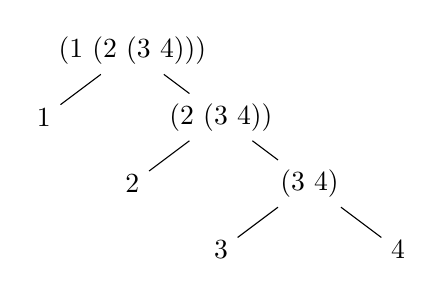
\begin{tikzpicture}[sibling distance=64pt, level distance=24pt]
\node{\lstinline{(1 (2 (3 4)))}}
  child{node{\lstinline{1}}}
  child{node{\lstinline{(2 (3 4))}}
    child{node{\lstinline{2}}}
    child{node{\lstinline{(3 4)}}
      child{node{\lstinline{3}}}
      child{node{\lstinline{4}}}}};
\end{tikzpicture}

\section{Exercise 2.25}

Code:

\begin{lstlisting}
(let ((l (list 1 3 (list 5 7) 9)))
  (car (cdr (car (cdr (cdr l))))))
(let ((l (list (list 7))))
  (car (car l)))
(let ((l (list 1 (list 2 (list 3 (list 4
  (list 5 (list 6 7))))))))
  (car (cdr (car (cdr (car (cdr (car (cdr
    (car (cdr (car (cdr l)))))))))))))
\end{lstlisting}

\section{Exercise 2.26}

The results are respectively
\lstinline{(1 2 3 4 5 6)},
\lstinline{((1 2 3) 4 5 6)},
and \lstinline{((1 2 3) (4 5 6))}.

\section{Exercise 2.27}

Code:

\begin{lstlisting}
(define (deep-reverse lst)
  (define (reverse-iter new lst)
    (define (reverse-elem elem)
      (if (list? elem)
          (reverse-iter (list) elem)
          elem))
    (if (null? lst)
        new
        (reverse-iter (cons (reverse-elem (car lst)) new) (cdr lst))))
  (reverse-iter (list) lst))
\end{lstlisting}

\section{Exercise 2.28}

Code:

\begin{lstlisting}
(define (fringe t)
  (if (list? t)
      (if (null? t)
          t
          (append (fringe (car t))
                  (fringe (cdr t))))
      (list t)))
\end{lstlisting}

\section{Exercise 2.29}

\subsection{a.}

Code:

\begin{lstlisting}
(define (left-branch mobile)
  (car mobile))
(define (right-branch mobile)
  (car (cdr mobile)))
(define (branch-length branch)
  (car branch))
(define (branch-structure branch)
  (car (cdr branch)))
\end{lstlisting}

\subsection{b.}

Code:

\begin{lstlisting}
(define (total-weight mobile)
  (+ (branch-weight (left-branch mobile))
     (branch-weight (right-branch mobile))))
\end{lstlisting}

\subsection{c.}

Methods to be rewritten:

\begin{lstlisting}
(define (right-branch mobile)
  (cdr mobile))
(define (branch-structure branch)
  (cdr branch))
\end{lstlisting}

\section{Exercise 2.30}

Code defining \lstinline{square-tree} directly:

\begin{lstlisting}
(define (square-tree t)
  (cond ((null? t) t)
        ((not (pair? t)) (* t t))
        (else (cons (square-tree (car t))
                    (square-tree (cdr t))))))
\end{lstlisting}

Code defining the same method using higher-order
 procedures:
 
\begin{lstlisting}
(define (square-tree t)
  (map (lambda (subtree)
         (if (pair? subtree)
           (square-tree subtree)
           (* subtree subtree)))
       t))
\end{lstlisting}

\section{Exercise 2.31}

Code:

\begin{lstlisting}
(define (tree-map method t)
  (map (lambda (subtree)
         (if (pair? subtree)
           (tree-map method subtree)
           (method subtree)))
       t))
\end{lstlisting}

\section{Exercise 2.32}

Code:

\begin{lstlisting}
(define (subsets s)
  (if (null? s)
      (list '())
      (let ((rest (subsets (cdr s))))
        (append rest (map (lambda (x)
                            (cons (car s) x))
                          rest)))))
\end{lstlisting}

\section{Exercise 2.33}

Code:

\begin{lstlisting}
(define (accumulate op initial seq)
  (if (null? seq)
      initial
      (op (car seq)
          (accumulate op initial (cdr seq)))))
(define (map p sequence)
  (accumulate (lambda (x y) (cons (p x) y)) (list) sequence))
(define (append seq1 seq2)
  (accumulate cons seq2 seq1))
(define (length sequence)
  (accumulate (lambda (x y) (+ 1 y)) 0 sequence))
\end{lstlisting}

\section{Exercise 2.34}

Code:

\begin{lstlisting}
(define (horner-eval x coefficient-sequence)
  (accumulate (lambda (this-coeff higher-terms)
                (+ this-coeff (* x higher-terms)))
              0
              coefficient-sequence))
\end{lstlisting}

\section{Exercise 2.35}

Code:

\begin{lstlisting}
(define (count-leaves t)
  (accumulate +
              0
              (map (lambda (subtree)
                     (if (not (pair? subtree))
                         1
                         (+ (count-leaves (car subtree))
                            (count-leaves (cdr subtree)))))
                   t)))
\end{lstlisting}

\section{Exercise 2.36}

Code:

\begin{lstlisting}
(define (accumulate-n op init seqs)
  (if (null? (car seqs))
    (list)
    (cons (accumulate op init (map car seqs))
          (accumulate-n op init (map cdr seqs)))))
\end{lstlisting}

\section{Exercise 2.37}

Code:

\begin{lstlisting}
(define (dot-product v w)
  (accumulate + 0 (map * v w)))
(define (matrix-*-vector mat vec)
  (map (lambda (row) (dot-product row vec)) mat))
(define (transpose mat)
  (accumulate-n cons (list) mat))
(define (matrix-*-matrix m n)
  (let ((cols (transpose n)))
    (map (lambda (row) (matrix-*-vector cols row)) m)))
\end{lstlisting}

\section{Exercise 2.38}

Result:

\begin{lstlisting}
3/2 ; 1/(2/(3/1))
1/6 ; ((1/1)/2)/3
(1 (2 (3 ())))
(((() 1) 2) 3)
\end{lstlisting}

The binary operation(procedure) \lstinline{op}
 should satisfy the commutative property for
 \lstinline{fold-left} and \lstinline{fold-right}
 to produce the same values for any sequence. Such
 operations include \lstinline{+}, \lstinline{*},
 etc.

\section{Exercise 2.39}

Code:

\begin{lstlisting}
(define (reverse sequence)
  (fold-right (lambda (curr result)
                (append result (list curr)))
              (list)
              sequence))
(define (reverse sequence)
  (fold-left (lambda (result curr)
               (cons curr result))
             (list)
             sequence))
\end{lstlisting}

\section{Exercise 2.40}

Code:

\begin{lstlisting}
(define (enumerate-interval start end)
  (define (enum-iter start end result)
    (if (> start end)
        result
        (enum-iter (+ start 1) end (append result (list start)))))
  (enum-iter start end (list)))
(define (unique-pairs n)
  (accumulate append
              (list)
              (map (lambda (i)
                     (map (lambda (j)
                            (list i j))
                          (enumerate-interval 1 (- i 1))))
                   (enumerate-interval 1 n))))
(define (prime-sum-pairs n)
  (map make-pair-sum
       (filter prime-sum? (unique-pairs n))))
\end{lstlisting}

\section{Exercise 2.41}

Code:

\begin{lstlisting}
(define (flatmap proc seq)
  (accumulate append (list) (map proc seq)))
(define (enumerate-triple-with-sum n)
  (flatmap append
           (map (lambda (i)
                  (map (lambda (j) (list i j (- n i j)))
                       (enumerate-interval 1 (- n i 1))))
                (enumerate-interval 1 (- n 2)))))
\end{lstlisting}

\section{Exercise 2.42}

Code:

\begin{lstlisting}
(define (queens board-size)
  (define empty-board (list))
  (define (get-row positions row)
    (list-ref positions (- (length positions) row)))
  (define (safe? k positions) ; is the last position (the kth) safe?
    (define (safe?-recur col1 col2)
      (define (safe?-test col1 col2)
        (let ((row1 (get-row positions col1))
              (row2 (get-row positions col2)))
          (not (or (= row1 row2)
                   (= (- col2 col1) (- row2 row1))
                   (= (- col1 col2) (- row2 row1))))))
      (cond ((= col1 col2) #t)
            ((safe?-test col1 col2) (safe?-recur (+ col1 1) col2))
            (else #f)))
    (safe?-recur 1 k))
  (define (adjoin-position new-row k rest-of-queens)
    (cons new-row rest-of-queens))
  (define (queen-cols k)
    (if (= k 0)
        (list empty-board)
        (filter
          (lambda (positions) (safe? k positions))
          (flatmap
            (lambda (rest-of-queens)
              (map (lambda (new-row)
                     (adjoin-position new-row k rest-of-queens))
                   (enumerate-interval 1 board-size)))
            (queen-cols (- k 1))))))
  (queen-cols board-size))
\end{lstlisting}

\section{Exercise 2.43}

Let $T(k)$ be the time needed by calling \lstinline{(queen-cols k)},
 $S(k)$ be the sum of combinations returned by
 \lstinline{(queen-cols k)}, $d$ be the size of board and
 $Q(k)$ be the time needed to check if one combination
 is valid. All operations that need constant time
 are denoted as 1s.

When calling \lstinline{(queen-cols k)} in the
 program in exercise 2.42, first \lstinline{(queen-cols (- k 1))}
 is called, which is time-consuming.
 It returns all combinations of the first $k-1$
 queens, each of which is later respectively appended
 with all possible column positions at the new row.
 Finally, all combinations, each of which consisting
 of $k$ queens, are evaluated and filtered to reserve
 only those without any checks.

According to the relation above, we have

\begin{align*}
T(k) &= T(k-1) + S(k-1) \cdot d \cdot Q(k) \\
&= T(k-2) + d \cdot \left[S(k-2) \cdot Q(k-1) + S(k-1) \cdot Q(k)\right] \\
&\vdots \\
&= T(0) + d \cdot \sum_{i=0}^{k-1} S(i) \cdot Q(i+1)
\end{align*}

On the contrary, when calling \lstinline{(queen-cols k)}
 in the program written by Louis, first all possible
 positions, with the sum of $d$, is generated. For each
 possible position, \lstinline{(queen-cols (- k 1))} is
 called and each of the combination returned is appended
 with the possible position in the new row. Finally,
 all combinations with the sum of $k$ queens are evaluated
 and filtered.

According to the relation above, we have

\begin{align*}
T'(k) &= d \cdot \left[T'(k-1) + S(k-1) \cdot Q(k)\right] \\
&= d \cdot T'(k-1) + S(k-1) \cdot d \cdot Q(k) \\
&= d^2 \cdot T'(k-2) + S(k-2) \cdot d^2 \cdot Q(k-1) + S(k-1) \cdot d \cdot Q(k) \\
&\vdots \\
&= d^k \cdot T'(0) + \sum_{i=0}^{k-1} d^{k-i} \cdot S(i) \cdot Q(i + 1)
\end{align*}

From which we have roughly

$$
T'(d) \approx d^d T(d)
$$

\section{Exercise 2.44}

Code:

\begin{lstlisting}
(define (up-split painter n)
  (if (= n 0)
      painter
      (let ((smaller (up-split painter (- n 1))))
        (below painter (beside smaller smaller)))))
\end{lstlisting}

\section{Exercise 2.45}

Code:

\begin{lstlisting}
(define (split op1 op2)
  (define (compound painter n)
    (if (= n 0)
        painter
        (let ((smaller (compound painter (- n 1))))
          (op1 painter (op2 smaller smaller))))))
\end{lstlisting}

\section{Exercise 2.46}

Code:

\begin{lstlisting}
(define (make-vect x y)
  (cons x y))
(define (xcor-vect vect)
  (car vect))
(define (ycor-vect vect)
  (cdr vect))
(define (add-vect vec1 vec2)
  (make-vect (+ (xcor-vect vec1) (xcor-vect vec2))
             (+ (ycor-vect vec1) (ycor-vect vec2))))
(define (sub-vect vec1 vec2)
  (make-vect (- (xcor-vect vec1) (xcor-vect vec2))
             (- (ycor-vect vec1) (ycor-vect vec2))))
(define (scale-vect factor vec)
  (make-vect (* factor (xcor-vect vec1))
             (* factor (ycor-vect vec2))))
\end{lstlisting}

\section{Exercise 2.47}

Selectors for the first implementation:

\begin{lstlisting}
(define (origin-frame frame)
  (list-ref frame 0))
(define (edge1-frame frame)
  (list-ref frame 1))
(define (edge2-frame frame)
  (list-ref frame 2))
\end{lstlisting}

Selectors for the second implementation:

\begin{lstlisting}
(define (origin-frame frame)
  (car frame))
(define (edge1-frame frame)
  (car (cdr frame)))
(define (edge2-frame frame)
  (cdr (cdr frame)))
\end{lstlisting}

\section{Exercise 2.48}

Code:

\begin{lstlisting}
(define (make-segment start end)
  (cons start end))
(define (start-segment segment)
  (car segment))
(define (end-segment segment)
  (cdr segment))
\end{lstlisting}

\section{Exercise 2.49}

Code:

\subsection{a.}

\begin{lstlisting}
(define frame-painter
  (let ((top-left (make-vect 0.0 1.0))
        (top-right (make-vect 1.0 1.0))
        (bottom-left (make-vect 0.0 0.0))
        (bottom-right (make-vect 1.0 0.0)))
    (segments->painter
      (list (make-segment top-left top-right)
            (make-segment top-right bottom-right)
            (make-segment bottom-right bottom-left)
            (make-segment bottom-left top-left)))))
\end{lstlisting}

\subsection{b.}

\begin{lstlisting}
(define X-painter
  (let ((top-left (make-vect 0.0 1.0))
        (top-right (make-vect 1.0 1.0))
        (bottom-left (make-vect 0.0 0.0))
        (bottom-right (make-vect 1.0 0.0)))
    (segments-painter
      (list (make-segment top-left bottom-right)
            (make-segment top-right bottom-left)))))
\end{lstlisting}

\subsection{c.}

\begin{lstlisting}
(define diamond-painter
  (let ((left (make-vect 0.0 0.5))
        (up (make-vect 0.5 1.0))
        (right (make-vect 1.0 0.5))
        (down (make-vect 0.5 0.0)))
    (segments-painter
      (list (make-segment left up)
            (make-segment up right)
            (make-segment right down)
            (make-segment down left)))))
\end{lstlisting}

\subsection{d.}

Omitted.

\section{Exercise 2.50}

Code:

\begin{lstlisting}
(define (flip-horiz painter)
  (transform-painter painter
                     (make-vect 1.0 0.0)
                     (make-vect 0.0 0.0)
                     (make-vect 1.0 1.0)))
(define (rotate-counter-180 painter)
  (transform-painter painter
                     (make-vect 1.0 1.0)
                     (make-vect 0.0 1.0)
                     (make-vect 1.0 0.0)))
(define (rotate-clock-90 painter)
  (transfrom-painter painter
                     (make-vect 0.0 1.0)
                     (make-vect 0.0 0.0)
                     (make-vect 1.0 1.0)))
\end{lstlisting}

\section{Exercise 2.51}

First version of code:

\begin{lstlisting}
(define (below painter1 painter2)
  (let ((paint-down
          (transform-painter painter1
                             (make-vect 0.0 0.0)
                             (make-vect 1.0 0.0)
                             (make-vect 0.0 0.5)))
        (paint-up
          (transform-painter painter2
                             (make-vect 0.0 0.5)
                             (make-vect 1.0 0.5)
                             (make-vect 0.0 1.0)))
    (lambda (frame)
      (paint-down frame)
      (paint-up frame)))))
\end{lstlisting}

Second version of code:

\begin{lstlisting}
(define (below painter1 painter2)
  (rotate-counter-90
    (beside (rotate-clock-90 painter1)
            (rotate-clock-90 painter2))))
\end{lstlisting}

\section{Exercise 2.52}

Code:

\subsection{a.}

Omitted.

\subsection{b.}

\begin{lstlisting}
(define (corner-split painter n)
  (if (= n 0)
      painter
      (let ((up (up-split painter (- n 1)))
            (right (right-split painter (- n 1))))
        (let ((top-left up)
              (bottom-right right)
              (corner (corner-split painter (- n 1)))))
          (beside (below painter top-left)
                  (below bottom-right corner)))))
\end{lstlisting}

\subsection{c.}

\begin{lstlisting}
(define (square-limit painter n)
  (let ((combine4 (square-of-four flip-horiz
                                  identity
                                  rotate180
                                  flip-vert)))
    (combine4 (corner-split (flip-vert painter) n))))
\end{lstlisting}

\section{Exercise 2.53}

Result:

\begin{lstlisting}
(a b c)
((george))
((y1 y2))
(y1 y2)
#f
#f
(red shoes blue socks)
\end{lstlisting}

\section{Exercise 2.54}

\begin{lstlisting}
(define (equal? stuff1 stuff2)
  (define (equal-list? list1 list2)
     (cond ((and (null? list1) (null? list2)) #t)
           ((or (null? list1) (null? list2)) #f)
           ((eq? (car list1) (car list2))
            (equal-list? (cdr list1) (cdr list2)))
           (else #f)))
  (cond ((and (list? stuff1) (list? stuff2))
         (equal-list? stuff1 stuff2))
        ((and (not (list? stuff1)) (not (list? stuff2)))
         (eq? stuff1 stuff2))
        (else #f)))
\end{lstlisting}

\section{Exercise 2.55}

\lstinline{'expr} is just an abbreviation of
 \lstinline{(quote expr)}, thus \lstinline{(car 'expr)}
 actually returns \lstinline{(car (quote expr))}.

In \lstinline{''abra...} where the expression itself
 is \lstinline{(quote abra...)}. The outer \lstinline{quote}
 prevents it from being evaluated, so it remains
 \lstinline{(quote abra...)} when passed to \lstinline{car},
 which returns \lstinline{quote}.

\section{Exercise 2.56}

Code:

\begin{lstlisting}
(define (deriv exp var)
  (cond ((number? exp) 0)
        ((variable? exp)
          (if (same-variable? exp var) 1 0))
        ((sum? exp)
          (make-sum (deriv (addend exp) var)
                    (deriv (augend exp) var)))
        ((product? exp)
          (make-sum
            (make-product (multiplier exp)
                          (deriv (multiplicand exp) var))
            (make-product (deriv (multiplier exp) var)
                          (multiplicand exp))))
        ((expo? exp)
          (make-product (make-product (exponent exp)
                                      (make-expo (base exp)
                                                 (make-sum (exponent exp)
                                                           -1)))
                        (deriv (base exp) var)))))
(define (expo? x)
  (and (pair? x) (eq? (car x) '**)))
(define (base x)
  (cadr x))
(define (exponent x)
  (caddr x))
(define (make-expo base exponent)
  (cond ((=number? exponent 0) 1)
        ((=number? base 0) 0)
        ((=number? exponent 1) base)
        (else (list '** base exponent))))
\end{lstlisting}

Definition of \lstinline{=number?}:

\begin{lstlisting}
(define (=number? exp num)
  (and (real? exp) (= exp num)))
\end{lstlisting}

\section{Exercise 2.57}

Code:

\begin{lstlisting}
(define (augend s)
  (if (= (length s) 3)
      (caddr s)
      (cons '+ (cddr s))))
(define (multiplicand p)
  (if (= (length p) 3)
      (caddr p)
      (cons '* (cddr p))))
\end{lstlisting}

\section{Exercise 2.58}

\subsection{a.}

This is quite simple actually, since
 nothing but only the relative positions
 are changed.

\subsection{b.}

First search the expression for \lstinline{+}.
 If \lstinline{+} is found, then compute
 differentials of both sides of the expression
 respectively and make summand of them.

If no \lstinline{+} is found, then select any
 one of the \lstinline{*}s, and regard both sides
 of the expression repectively as the multiplier
 and the multiplicand, so as to apply the rule
 for products.

\section{Exercise 2.59}

Code:

\begin{lstlisting}
(define (union-set set1 set2)
  (cond ((or (null? set1) (null? set2))
         (append set1 set2))
        ((element-of-set? (car set1) set2)
         (union-set (cdr set1) set2))
        (else (cons (car set1)
                    (union-set (cdr set1) set2)))))
\end{lstlisting}

\section{Exercise 2.60}

Code:

\begin{lstlisting}
(define (element-of-set? x set)
  (cond ((null? set) #f)
        ((equal? x (car set)) #t)
        (else (element-of-set? x (cdr set)))))
(define (adjoin-set x set)
  (cons x set))
(define (union-set set1 set2)
  (append set1 set2))
(define (intersection-set set1 set2)
  (cond ((or (null? set1) (null? set2)) '())
        ((element-of-set? (car set1) set2)
         (cons (car set1)
               (intersection-set (cdr set1) set2)))
        (else (intersection-set (cdr set1) set2))))
\end{lstlisting}

The \lstinline{element-of-set?} and
 \lstinline{intersection-set} operations
 can be much more time consuming, while the
 \lstinline{adjoin-set} and \lstinline{union-set}
 operations are much more efficient.
 Applications dealing with sparse elements
 may prefer this representation, since they
 don't bring about too much duplication and
 at the same time are much efficient when
 doing \lstinline{adjoin-set} and \lstinline{union-set}.

\section{Exercise 2.61}

Code:

\begin{lstlisting}
(define (adjoin-set x set)
  (define (adjoin-set-iter result x rest)
    (cond ((null? rest) (append set (list x)))
          ((= (car rest) x) set)
          ((< (car rest) x)
           (adjoin-set-iter (append result (list (car rest)))
                            x
                            (cdr rest)))
          (else (append result (list x) rest))))
  (adjoin-set-iter '() x set))
\end{lstlisting}

Suppose there are $n$ elements already in the set
 before adjoining $x$ into the set. In average case
 about half the elements (i.e. $\frac{n}{2}$ elements)
 are smaller than $x$ and the other half are larger
 than $x$. Therefore on average only $\frac{n}{2}$
 iterations are needed.

As for the unordered representation, every time
 \lstinline{adjoin-set} is carried out iterations
 (with a total of $n$)
 through the whole set must be done to ensure
 that no duplication exists.

\section{Exercise 2.63}

\subsection{a.}

They do.

Result:

\begin{lstlisting}
(1 3 5 7 9 11)
\end{lstlisting}

\subsection{b.}

The time consumption of the first procedure,
 denoted as $T_1(n)$, satisfies the following
 equation:

\begin{align*}
&T_1(n) = 2T_1\left(\frac{n}{2}\right) + \Theta(n) \\
\implies &T_1(n) = \Theta(n\log n)
\end{align*}

For the second procedure:

\begin{align*}
&T_2(n) = 2T_2\left(\frac{n}{2}\right) + C \\
\implies &T_2(n) = \Theta(n)
\end{align*}

\section{Exercise 2.64}

\subsection{a.}

First, consider whether the length of list
 to be converted is 0. If so, just return
 an empty tree and the list unmodified.

If not, then select one element around the center
 of the interval, and recursively convert
 the left part and the right part as two subtrees.
 Finally return this tree and remaining part
 of list.

The tree produced by \lstinline{list->tree}:

\vspace{2mm}

\tikzset{sibling distance=24pt, level distance=24pt}
\Tree
[.{5}
	[.{1}
		\edge[draw=none];{}
		{3}
	]
	[.{9}
		{7}
		{11}
	]
]

\subsection{b.}

Let the time taken to convert a list of $n$
 be $T(n)$, then we have

\begin{align*}
&T(n) = 2T\left(\frac{n}{2}\right) + C \\
\implies &T(n) = \Theta(n)
\end{align*}

\section{Exercise 2.65}

Code:

\begin{lstlisting}
(define (union-set set1 set2)
  (let ((list1 (tree->list set1))
        (list2 (tree->list set2)))
    (list->tree (union-list list1 list2))))
(define (intersection-set set1 set2)
  (let ((list1 (tree->list set1))
        (list2 (tree->list set2)))
    (list->tree (intersection-list list1 list2))))
\end{lstlisting}

Let the size of \lstinline{set1} and \lstinline{set2}
 be both $n$, then converting them to lists, doing
 union/intersection and converting the final list back
 to set each takes $\Theta(n)$ time, thus the entire
 procedure is $\Theta(n)$ growth.

\section{Exercise 2.66}

Code:

\begin{lstlisting}
(define (lookup given-key set-of-records)
  (cond ((null? set-of-records) false)
        ((equal? given-key (key (entry set-of-records)))
         (entry set-of-records))
        (else (let ((left-result (lookup given-key
                                         (left-branch set-of-records))))
                (if (equal? left-result false)
                    false
                    (lookup given-key
                            (right-branch set-of-records)))))))
\end{lstlisting}

\section{Exercise 2.67}

Result: ADABBCA

\section{Exercise 2.68}

Code:

\begin{lstlisting}
(define (encode-symbol symbol tree)
  (define (encode-iter symbol tree result)
    (if (leaf? tree)
        (if (eq? (symbol-leaf tree) symbol)
            result
            '())
        (append (encode-iter symbol
                             (left-branch tree)
                             (append result '(0)))
                (encode-iter symbol
                             (right-branch tree)
                             (append result '(1))))))
  (encode-iter symbol tree '()))
\end{lstlisting}

\section{Exercise 2.69}

Code:

\begin{lstlisting}
(define (successive-merge leaf-set)
  (if (null? (cdr leaf-set))
      (car leaf-set)
      (successive-merge
        (adjoin-set
          (make-code-tree (car leaf-set)
                          (cadr leaf-set))
          (cddr leaf-set)))))
\end{lstlisting}

\section{Exercise 2.70}

Complete version of code:

\begin{lstlisting}
; leaf definition
(define (make-leaf symbol weight)
  (list 'leaf symbol weight))
(define (leaf? object)
  (eq? (car object) 'leaf))
(define (symbol-leaf x) (cadr x))
(define (weight-leaf x) (caddr x))

; tree definition
(define (make-code-tree left right)
  (list left
        right
        (append (symbols left) (symbols right))
        (+ (weight left) (weight right))))
(define (left-branch tree) (car tree))
(define (right-branch tree) (cadr tree))
(define (symbols tree)
  (if (leaf? tree)
      (list (symbol-leaf tree))
      (caddr tree)))
(define (weight tree)
  (if (leaf? tree)
      (weight-leaf tree)
      (cadddr tree)))

; leaf set definition
(define (adjoin-set x set)
  (cond ((null? set) (list x))
        ((< (weight x) (weight (car set)))
         (cons x set))
        (else (cons (car set)
                    (adjoin-set x (cdr set))))))
(define (make-leaf-set pairs)
  (if (null? pairs)
      '()
      (let ((pair (car pairs)))
        (adjoin-set (make-leaf (car pair)
                               (cadr pair))
                    (make-leaf-set (cdr pairs))))))

; tree-generating method definition
(define (generate-huffman-tree pairs)
  (define (successive-merge leaf-set)
    (if (null? (cdr leaf-set))
        (car leaf-set)
        (successive-merge
          (adjoin-set
            (make-code-tree (car leaf-set)
                            (cadr leaf-set))
            (cddr leaf-set)))))
  (successive-merge (make-leaf-set pairs)))

; encode method definition
(define (encode-symbol symbol tree)
  (define (encode-iter symbol tree result)
    (if (leaf? tree)
        (if (eq? (symbol-leaf tree) symbol)
            result
            '())
        (append (encode-iter symbol
                             (left-branch tree)
                             (append result '(0)))
                (encode-iter symbol
                             (right-branch tree)
                             (append result '(1))))))
  (encode-iter symbol tree '()))
(define (encode message tree)
  (if (null? message)
      '()
      (append (encode-symbol (car message) tree)
              (encode (cdr message) tree))))

; tree generation
(define rock-tree
  (generate-huffman-tree (list '(A 2)
                               '(BOOM 1)
                               '(GET 2)
                               '(JOB 2)
                               '(NA 16)
                               '(SHA 3)
                               '(YIP 9)
                               '(WAH 1))))

; encode
(encode '(GET A JOB
          SHA NA NA NA NA NA NA NA NA
          GET A JOB
          SHA NA NA NA NA NA NA NA NA
          WAH YIP YIP YIP YIP YIP YIP YIP YIP YIP
          SHA BOOM) rock-tree)
\end{lstlisting}

Result:

\begin{lstlisting}
(1 1 1 1 1 1 1 0 0 1
 1 1 1 0 1 1 1 0 0 0
 0 0 0 0 0 0 1 1 1 1
 1 1 1 0 0 1 1 1 1 0
 1 1 1 0 0 0 0 0 0 0
 0 0 1 1 0 1 0 1 0 1
 0 1 0 1 0 1 0 1 0 1
 0 1 0 1 0 1 1 1 0 1
 1 0 1 1)
\end{lstlisting}

It takes 84 bits to encode the 36 symbols.
 On the contrary it takes 108 bits using fixed-length
 code (3 bits each symbol).

\section{Exercise 2.71}

Let the symbols be $s_0, s_1, s_2 \cdots$ and
 the symbol $s_i$ has the relative frequency
 $2^i$, then one possible structure of Huffman
 tree is like:

\tikzset{sibling distance=24pt, level distance=24pt}
\Tree
[.{}
	{$s_{n-1}$}
	[.{}
		{$s_{n-2}$}
		[.{}
			{$s_{n-3}$}
			{$\cdots$}
		]
	]
]

For $n=10$, it takes $1$ bit to encode the most
 frequent symbol, and $n-1$ bits to encode the lease
 frequent one.

\section{Exercise 2.72}

To reduce the time of comparing target symbol
 to others, my algorithm does the comparison
 only when visiting a leaf. It traverses through
 the whole tree, with only the right leaf returning
 the code, and the wrong ones returning an empty
 list.

Encoding both the most frequent symbol and the lease
frequent symbol takes $\Theta(n)$ time.

\section{Complete code in section 2.4.3}

\begin{lstlisting}
; code offering type support
(define (attach-tag type-tag contents)
  (cons type-tag contents))
(define (type-tag datum)
  (if (pair? datum)
      (car datum)
      (error "bad tagged datum" datum)))
(define (contents datum)
  (if (pair? datum)
      (cdr datum)
      (error "bad tagged datum" datum)))
(define (make-table)
  (let ((local-table (list 'table)))
    (define (lookup key1 key2)
      (let ((subtable (assoc key1 (cdr local-table))))
        (if subtable
            (let ((record (assoc key2 (cdr subtable))))
              (if record
                  (cdr record)
                  false))
            false)))
    (define (insert! key1 key2 value)
      (let ((subtable (assoc key1 (cdr local-table))))
        (if subtable
            (let ((record (assoc key2 (cdr subtable))))
              (if record
                  (set-cdr! record value)
                  (set-cdr! subtable
                            (cons (cons key2 value)
                                  (cdr subtable)))))
            (let ((new-subtable (list key1 (cons key2 value))))
              (set-cdr! local-table
                        (cons new-subtable
                              (cdr local-table))))))
      'ok)
    (define (dispatch method-name)
      (cond ((eq? method-name 'lookup) lookup)
            ((eq? method-name 'insert!) insert!)
            (else (error "unknown method" method-name))))
    dispatch))
(define operation-table (make-table))
(define get (operation-table 'lookup))
(define put (operation-table 'insert!))
(define (apply-generic op . args)
  (let ((type-tags (map type-tag args)))
    (let ((proc (get op type-tags)))
      (if proc
          (apply proc (map contents args))
          (error "no method available"
                 (list op type-tags))))))

; type-dependent primitive operations
(define (rectangular? z)
  (eq? (type-tag z) 'rectangular))
(define (polar? z)
  (eq? (type-tag z) 'polar))
(define (install-rectangular-package)
  ; internal representation: (real-part, imag-part)
  (define (real-part z) (car z))
  (define (imag-part z) (cdr z))
  (define (magnitude z)
    (sqrt (+ (square (real-part z))
             (square (imag-part z)))))
  (define (angle z)
    (atan (imag-part z) (real-part z)))
  (define (make-from-real-imag x y) (cons x y))
  (define (make-from-mag-ang r a)
    (cons (* r (cos a)) (* r (sin a))))
  (define (tag x) (attach-tag 'rectangular x))
  (put 'real-part '(rectangular) real-part)
  (put 'imag-part '(rectangular) imag-part)
  (put 'magnitude '(rectangular) magnitude)
  (put 'angle '(rectangular) angle)
  (put 'make-from-real-imag '(rectangular)
    (lambda (x y) (tag (make-from-real-imag x y))))
  (put 'make-from-mag-ang '(rectangular)
    (lambda (r a) (tag (make-from-mag-ang r a))))
  'done)
(define (install-polar-package)
  ; internal representation: (magnitude, angle)
  (define (magnitude z) (car z))
  (define (angle z) (cdr z))
  (define (real-part z)
    (* (magnitude z) (cos (angle z))))
  (define (imag-part z)
    (* (magnitude z) (sin (angle z))))
  (define (make-from-mag-ang r a) (cons r a))
  (define (make-from-real-imag x y)
    (cons (sqrt (+ (square x) (square y)))
          (atan y x)))
  (define (tag x) (attach-tag 'polar x))
  (put 'real-part '(polar) real-part)
  (put 'imag-part '(polar) imag-part)
  (put 'magnitude '(polar) magnitude)
  (put 'angle '(polar) angle)
  (put 'make-from-real-imag '(polar)
    (lambda (x y) (tag (make-from-real-imag x y))))
  (put 'make-from-mag-ang '(polar)
    (lambda (r a) (tag (make-from-mag-ang r a))))
  'done)

; type-independent primitive operations
(define (make-from-real-imag x y)
  ((get 'make-from-real-imag '(rectangular)) x y))
(define (make-from-mag-ang r a)
  ((get 'make-from-mag-ang '(polar)) r a))
(define (real-part z)
  (apply-generic 'real-part z))
(define (imag-part z)
  (apply-generic 'imag-part z))
(define (magnitude z)
  (apply-generic 'magnitude z))
(define (angle z)
  (apply-generic 'angle z))
(define (add-complex z1 z2)
  (make-from-real-imag (+ (real-part z1) (real-part z2))
                       (+ (imag-part z1) (imag-part z2))))
(define (sub-complex z1 z2)
  (make-from-real-imag (- (real-part z1) (real-part z2))
                       (- (imag-part z1) (imag-part z2))))
(define (mul-complex z1 z2)
  (make-from-mag-ang (* (magnitude z1) (magnitude z2))
                     (+ (angle z1) (angle z2))))
(define (div-complex z1 z2)
  (make-from-mag-ang (/ (magnitude z1) (magnitude z2))
                     (- (angle z1) (angle z2))))
\end{lstlisting}

\section{Exercise 2.73}

\subsection{a.}

When calling \lstinline{deriv}, tell if the given
 expression is a number or a variable. If so, apply
 to corresponding rule to the expression. Elsewise,
 get the corresponding derivative handler to the
 operator, then apply it to the operands.

For numbers and variables, \lstinline{(car exp)} returns
 the single number/variable, which is not operator and
 shouldn't be passed to \lstinline{get}  expecting
 a type instead of a value.

\subsection{b.}

Code:

\begin{lstlisting}
(define (deriv-sum exp var)
  (make-sum (deriv (addend exp) var)
            (deriv (augend exp) var)))
(define (deriv-product exp var)
  (make-sum
    (make-product (multiplier exp)
                  (deriv (multiplicand exp) var))
    (make-product (deriv (multiplier exp) var)
                  (multiplicand exp))))
(put 'deriv '(+) deriv-sum)
(put 'deriv '(*) deriv-product)
\end{lstlisting}

\subsection{c.}

Code:

\begin{lstlisting}
(define (deriv-expo exp var)
  (make-product (make-product (exponent exp)
                              (make-expo (base exp)
                                         (make-sum (exponent exp)
                                                   -1)))
                (deriv (base exp) var)))
(put 'deriv '(**) deriv-expo)
\end{lstlisting}

\subsection{d.}

Simply exchange the first two arguments when calling
 \lstinline{put}.
 
\section{Exercise 2.74}

\subsection{a.}

Code:

\begin{lstlisting}
(define (get-record file employee)
   ((get 'get-record (division file)) (content file) employee))
\end{lstlisting}

Each division should implement its own
 \lstinline{get-record} method and install
 it in the table. The file should be tagged
 with division identifier (using the same
 procedure as every other division).

\subsection{b.}

Code:

\begin{lstlisting}
(define (get-salary record)
  ((get 'get-salary (division record)) (content record)))
\end{lstlisting}

Each division should implement its own
 \lstinline{get-salary} method and install
 it in the table. The record should be tagged
 with division identifier.

\subsection{c.}

Code:

\begin{lstlisting}
(define (find-employee-record employee file-list)
  (if (null? file-list)
      '()
      (let ((curr-result (get-record (car file-list)
                                     employee)))
        (if (null? curr-result)
            (find-employee-record employee (cdr file-list))
            curr-result))))
\end{lstlisting}

\subsection{d.}

Type information now consists of company identifier
 and division identifier. All entries in the table
 must be updated.

\section{Exercise 2.75}

Code:

\begin{lstlisting}
(define (make-from-mag-ang mag ang)
  (define (dispatch op)
    (cond ((eq? op 'real-part) 
            (* mag (cos ang)))
          ((eq? op 'imag-part)
            (* mag (sin ang)))
          ((eq? op 'magnitude) mag)
          ((eq? op 'angle) ang)
          (else
            (error "Unknown op -- MAKE-FROM-MAG-ANG" op))))
  dispatch)
\end{lstlisting}

Tests:

\begin{lstlisting}
(= ((make-from-mag-ang 1 2) 'magnitude) 1) ; #t expected
(= ((make-from-mag-ang 1 2) 'angle) 2) ; #t expected
((make-from-mag-ang 1 1.571) 'real-part) ; approximately 0 expected
((make-from-mag-ang 1 1.571) 'imag-part) ; approximately 1 expected
\end{lstlisting}

Result:

\begin{lstlisting}
#t ; pass
#t ; pass
-2.0367320369517789e-4 ; pass
.9999999792586128 ; pass
\end{lstlisting}

\section{Exercise 2.76}

When using generic operations with explicit
 dispatch:

\begin{itemize}
\item When new types are added, all
 operations need to be modified to adapt to
 new types.
\item When new operations are added, the
 new operation need to explicitly handle
 every data type. No modifications are
 needed for the original part.
\end{itemize}

When using data-directed style:

\begin{itemize}
\item When new types are added, new columns
 are added to the table. Each column corresponds to
 all operations of a particular type.
\item When new operations are added, new
 rows are added to the table. Each row corresponds to
 all types supporting a particular operation.
\end{itemize}

When using message-passing style:

\begin{itemize}
\item When new types are added, the type definition
 and all operations each type supports are added.
 No modifications are needed for the original part.
\item When new operations are added, all
 original type definitions need to be modified
 to support new operations.
\end{itemize}

The second and third style are the most appropriate
 ones for a system in which new types must be often added.
 The first and second style are the most appropriate
 ones for a system in which new operations must be often
 added.

\section{Exercise 2.77}

Evaluation procedure is as below:

\begin{lstlisting}
(magnitude (complex rectangular 3 . 4)) ->
(apply-generic 'magnitude (complex rectangular 3 . 4)) ->
(magnitude (rectangular 3 . 4)) ->
(apply-generic 'magnitude (rectangular 3 . 4)) ->
25
\end{lstlisting}

When \lstinline{apply-generic} get invoked for the first time,
 \lstinline{magnitude} is dispatched to according to tag
 \lstinline{complex}. Then \lstinline{apply-generic} get invoked
 for the second time, when the actual \lstinline{magitude}
 procedure for \lstinline{rectangle} numbers is dispatched to.

\section{Exercise 2.78}

Code:

\begin{lstlisting}
(define (type-tag datum)
  (cond ((pair? datum) (car datum))
        ((number? datum) 'scheme-number)
        (else (error "Bad tagged datum -- TYPE-TAG" datum))))
(define (contents datum)
  (cond ((pair? datum) (cdr datum))
        ((number? datum) datum)
        (else (error "Bad tagged datum -- CONTENTS" datum))))
(define (attach-tag type-tag contents)
  (if (number? contents)
      contents
      (cons type-tag contents)))
\end{lstlisting}

\section{Exercise 2.79}

Code:

\begin{lstlisting}
(put 'equ? '(scheme-number scheme-number)
  (lambda (x y) (= x y)))
(put 'equ? '(rational rational)
  (lambda (x y) (and (= (numer x) (numer y))
                     (= (denom x) (denom y)))))
(put 'equ? '(complex complex)
  (lambda (x y) (and (= (real-part x) (real-part y))
                     (= (imag-part y) (imag-part y)))))
(define (equ? x y)
  (apply-generic 'equ? x y))
\end{lstlisting}

\section{Exercise 2.80}

Code:

\begin{lstlisting}
(put '=zero? '(scheme-number)
  (lambda (x) (= x 0)))
(put '=zero? '(rational)
  (lambda (x) (= (numer x) 0)))
(put '=zero? '(complex)
  (lambda (x) (and (= (real-part x) 0)
                   (= (imag-part x) 0))))
(define (=zero? x)
  (apply-generic '=zero? x))
\end{lstlisting}

\section{Exercise 2.81}

\subsection{a.}

Since the operation is not in the table, the program
 would apply coersions to each of the operands, and make
 another call of \lstinline{apply-generic} with the
 same operands still with the same type, causing an
 infinite loop in the end.

\subsection{b.}

Louis is wrong, but something could be done, indeed.

Suppose we've implemented complex numbers and operations
 including addition and subtraction. Now when we implement
 integers, we don't necessarily need to implement
 addition and substraction again, since all integers can
 be converted to complex numbers and be applied with
 the operations of the complex numbers. Therefore, if
 the program finds that there's no available operation
 for two objects with the same type, it would be good
 if it can look up in the type hierarchy for a common
 supertype where the operation is available.

\subsection{c.}

Code:

\begin{lstlisting}
(define (apply-generic op . args)
  (let ((type-tags (map type-tag args)))
    (let ((proc (get op type-tags)))
      (if proc
          (apply proc (map contents args))
          (if (= length args) 2)
              (let ((type1 (car type-tags))
                    (type2 (cadr type-tags))
                    (a1 (car args))
                    (a2 (cadr args)))
                (if (eq? type1 type2)
                    (error "No method for type" (list op type1))
                    (let ((t1->t2 (get-coercion type1 type2))
                          (t2->t1 (get-coercion type2 type1)))
                      (cond (t1->t2
                              (apply-generic op (t1->t2 a1) a2))
                            (t2->t1
                              (apply-generic op a1 (t2->t1 a2)))
                            (else
                              (error "No method for types" (list op type-tags)))))))
              (error "No method for types" (list op type-tags))))))
\end{lstlisting}

\section{Exercise 2.82}

First to prove that the given strategy is not sufficiently general, suppose
 there are 3 arguments with type (B, B, A), where A is the supertype
 of B. Now using the given strategy, the combination of (A, B, A) or (B, A, A)
 will never be tried.

To try every combination is actually to traverse a directed graph. Each node
 represents a combination of types, and there's edge from one node to another
 if the former combination can be transformed to the latter with a single
 coercion. One fact about the graph is that there's only one node with the
 indegree of 0 (the original combination) and only one node with the outdegree
 of 0 (can't be coerced anymore). By performing a search (like BFS) on the graph
 starting from the original combination, one can always find an available
 combination if there is one.

\section{Exercise 2.83}

Code:

\begin{lstlisting}
(put 'raise '(integer)
  (lambda (x) (make-rational (contents x) 1)))
(put 'raise '(rational)
  (lambda (x)
          (let ((n (numer x))
                (d (denom x)))
            (make-real (/ n d)))))
(put 'raise '(real)
  (lambda (x) (make-complex (contents real) 0)))
(define (raise x)
  (apply-generic 'raise x))
\end{lstlisting}

\section{Exercise 2.84}

Code:

\begin{lstlisting}
(define (install-level-package)
  (put 'level 'integer 0)
  (put 'level 'rational 1)
  (put 'level 'real 2)
  (put 'level 'complex 3))
(define (operand-level op)
  (get 'level (type-tag op)))
(define (is-super? op1 op2)
  (> (operand-level op1)
     (operand-level op2)))
(define (apply-generic op . args)
  (let ((type-tags (map type-tag args)))
    (let ((proc (get op type-tags)))
      (if proc
          (apply proc (map contents args)
          (if (= (length args) 2)
            (let ((a1 (car args))
                  (a2 (cadr args)))
              (cond ((is-super? a1 a2) (apply-generic op a1 (raise a2)))
                    ((is-super? a2 a1) (apply-generic op (raise a1) a2))
                    (else (error "No method for these types"
                                 (list op type-tags)))))
            (error "No method for these types"
                   (list op type-tags))))))))
\end{lstlisting}

\section{Exercise 2.85}

Code:

\begin{lstlisting}
(define (drop n)
  (if (equal-generic? (raise (project n))
                      n)
      (drop (project n))
      n)))
\end{lstlisting}

This topic has been on for a really long period. I Really
 want to speed up so a lot of code is omitted.

\section{Exercise 2.86}

It's been a long time since the last time I tested my code.
 Honestly, writing code that can't run is really frustrating.
 There's still a lot to go, and all the code can't run without
 \lstinline{put} and \lstinline{get}. Now I'm done with it
 and I'm gonna implement these two method before going on.
 Besides, to simplify the work, only two types and three operations
 are involved.

Complete version of code:

\begin{lstlisting}
(define (make-table)
  (let ((local-table (list '**table**)))
    (define (assoc key records)
      (cond ((null? records) #f)
            ((equal? key (caar records)) (car records))
            (else (assoc key (cdr records)))))
    (define (lookup key1 key2)
      (let ((subtable (assoc key1 (cdr local-table))))
        (if subtable
            (let ((record (assoc key2 (cdr subtable))))
              (if record
                  (cdr record)
                  false))
            false)))
    (define (insert! key1 key2 value)
      (let ((subtable (assoc key1 (cdr local-table))))
        (if subtable
            (let ((record (assoc key2 (cdr subtable))))
              (if record
                  (set-cdr! record value)
                  (set-cdr! subtable
                            (cons (cons key2 value)
                                  (cdr subtable)))))
            (set-cdr! local-table
                      (cons (list key1
                                  (cons key2 value))
                            (cdr local-table)))))
      'ok)
    (define (dispatch method)
      (cond ((eq? method 'lookup-proc) lookup)
            ((eq? method 'insert-proc) insert!)
            (else (error "No such method" method))))
    dispatch))

(define op-table (make-table))
(define put (op-table 'insert-proc))
(define get (op-table 'lookup-proc))

(define (attach-tag tag x)
  (if (number? x)
      x
      (cons tag x)))
(define (get-tag x)
  (if (number? x)
      'real
      (car x)))
(define (get-content x)
  (if (number? x)
      x
      (cdr x)))

(define (apply-generic op . args)
  (let ((type-tags (map get-tag args)))
    (let ((proc (get op type-tags)))
      (if proc
          (apply proc (map get-content args))
          (error "No method for" (list op type-tags))))))

(define (make type-tag . args)
  (apply (get 'make type-tag) args))
(define (add x y)
  (apply-generic 'add x y))
(define (mul x y)
  (apply-generic 'mul x y))
(define (display x)
  (apply-generic 'display x))

(define (install-real-package)
  (define (tag x)
    (attach-tag 'real x))
  (put 'make '(real)
       (lambda (x) (tag x)))
  (put 'add '(real real)
       (lambda (x y) (tag (+ x y))))
  (put 'mul '(real real)
       (lambda (x y) (tag (* x y))))
  (put 'display '(real)
       (lambda (x) (write x)))
  'ok)
(install-real-package)
(define (make-real x)
  (make '(real) x))

(define (install-rational-package)
  (define (tag x)
    (attach-tag 'rational x))
  (put 'make '(rational)
       (lambda (n d) (tag (cons n d))))
  (put 'add '(rational rational)
       (lambda (x y)
         (tag (cons (add (mul (car x) (cdr y))
                         (mul (cdr x) (car y)))
                    (mul (cdr x) (cdr y))))))
  (put 'mul '(rational rational)
       (lambda (x y)
         (tag (cons (mul (car x) (car y))
                    (mul (cdr x) (cdr y))))))
  (put 'display '(rational)
       (lambda (x) (write-string "(")
                   (display (car x))
                   (write-string ")/(")
                   (display (cdr x))
                   (write-string ")")))
  'ok)
(install-rational-package)
(define (make-rational n d)
  (make '(rational) n d))
\end{lstlisting}

The key difference from the former version of operations
 is that manipulations on components of numbers now need
 to invoke generic operations.

\section{Exercise 2.87}

Code:

\begin{lstlisting}
(put '=zero? 'polynomial
  (lambda (x) (null? (term-list x))))
\end{lstlisting}

\section{Exercise 2.88}

Code:

\begin{lstlisting}
(define (nega-term term)
  (make-term (order term)
             (nega (coeff term))))
(define (nega-terms term-list)
  (if (null? term-list)
      '()
      (cons (nega-term (car term-list)) (cdr term-list))))
(define (sub-terms L1 L2)
  (cond ((empty-termlist? L1) (nega-terms L2))
        ((empty-termlist> L2) L1)
        (else
          (let ((t1 (first-term L1))
                (t2 (first-term L2)))
            (cond ((> (order t1) (order t2))
                   (adjoin-term t1
                                (sub-terms (rest-terms L1) L2)))
                  ((< (order t1) (order t2))
                   (adjoin-term (nega-term t2)
                                (sub-terms L1 (rest-terms L2))))
                  (else
                    (adjoin-term
                      (make-term (order t1)
                                 (sub (coeff t1) (coeff t2)))
                      (sub-terms (rest-terms L1) (rest-terms L2)))))))))
(define (sub-poly p1 p2)
  (if (same-variable? (variable p1) (variable p2))
      (make-poly (variable p1)
                 (sub-terms (term-list p1)
                            (term-list p2)))
      (error "Polys not in same var -- SUB-POLY"
             (list p1 p2))))
(put 'sub '(polynomial polynomial)
     (lambda (p1 p2) (tag (sub-poly p1 p2))))
\end{lstlisting}

\section{Exercise 2.89}

Code:

\begin{lstlisting}
(define (install-polynomial-package)
  (define (add-poly p1 p2)
    (define (add-terms p1 p2)
      (if (null? p1)
          '()
          (cons (+ (car p1) (car p2))
                (add-terms (cdr p1) (cdr p2)))))
    (cond ((> (length p1) (length p2)) (add-poly p1 (cons 0 p2)))
          ((< (length p1) (length p2)) (add-poly (cons 0 p1) p2))
          (else (add-terms p1 p2))))
  (define (mul-poly p1 p2)
    (define (make-zero-list length)
      (if (= length 0)
          '()
          (cons 0 (make-zero-list (- length 1)))))
    (let ((first (car p1)))
         (if (null? (cdr p1))
             (map (lambda (x) (* x first)) p2)
             (add-poly (append (map (lambda (x) (* x first)) p2) (make-zero-list (- (length p1) 1)))
                       (mul-poly (cdr p1) p2)))))
  (define (tag p) (attach-tag 'polynomial p))
  (put 'make '(polynomial)
       (lambda (terms) (tag terms)))
  (put 'add '(polynomial polynomial)
       (lambda (p1 p2) (tag (add-poly p1 p2))))
  (put 'mul '(polynomial polynomial)
       (lambda (p1 p2) (tag (mul-poly p1 p2))))
\end{lstlisting}

\section{Exercise 2.90}

One way of doing this is to keep two exising packages
 (with different tags, of course) and to
 add an additional \lstinline{polynomial} tag.
 All method calls will be dispatched twice before
 invoking the actual method.

\section{Exercise 2.91}

Code:

\begin{lstlisting}
(define (div-terms L1 L2)
  (if (empty-termlist? L1)
      (list (the-empty-termlist) (the-empty-termlist))
      (let ((t1 (first-term L1))
            (t2 (first-term L2)))
        (if (> (order t2) (order t1))
            (list (the-empty-termlist) L1)
            (let ((new-coeff (div (coeff t1) (coeff t2)))
                  (new-order (- (order t1) (order t2))))
              (let ((rest-of-result
                     (div-terms (sub-terms L1
                                           (mul-terms L2
                                                      (list
                                                        (make-term new-order new-coeff))))
                                L2)))
                (list (cons (make-term new-order new-coeff)
                            (car rest-of-result))
                      (cdr rest-of-result))))))))
\end{lstlisting}

\section{Exercise 2.92}

\end{document}










